\documentclass[a4paper,12pt,hidelinks]{article}

\usepackage[T1]{fontenc}
\usepackage[utf8]{inputenc}
\usepackage[catalan]{babel}
\usepackage{blindtext}
\usepackage{graphicx}
\usepackage{wrapfig}
\usepackage{enumitem}
\usepackage{fancyhdr}
\usepackage{amsmath}
\usepackage{parskip}
\usepackage{microtype}
\usepackage{hyperref}
\usepackage{hypcap}
\usepackage{caption}
\usepackage{subcaption}

\hypersetup{pdftex,colorlinks=false}

\parskip 12pt

\begin{document}

    \title{\Large{\textbf{Projecte 1: Navegació}}}
    \author{Oscar Lostes Cazorla, 1458082\\
    Esteve Pineda Sánchez, 1455249\\
    Máximo Martínez Alcivar, 1455249}
    \date{31 de Març, 2019}

    \maketitle

    \begin{figure}[hb]    
        \centering  
        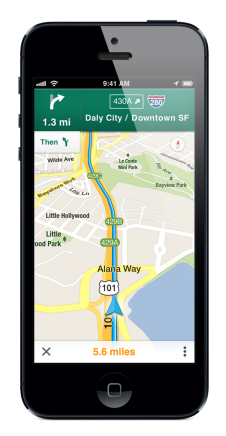
\includegraphics{portada.png}
    \end{figure}

    \thispagestyle{empty}

    \let\cleardoublepage\clearpage

    \pagebreak

    \setcounter{page}{1}

    \tableofcontents

    \pagestyle{fancy}
    \fancyhf{}
    \renewcommand{\headrulewidth}{2pt}
    \renewcommand{\footrulewidth}{1pt}

    \fancyhead[L]{Projecte 1: Navegació}
    \fancyhead[R]{Intel·ligència Artificial}
    \fancyfoot[C]{\thepage}

    \pagebreak

    \part{Introducció}
    \label{part:intro}

        L’objectiu d’aquesta pràctica és resoldre un problema ben habitual: com arribar del punt \textit{A} al \textit{B} de la millor forma possible. A diari emprem eines com \textit{Google Maps} per aquesta finalitat, i el que volem és fer una petita réplica aplicant els coneixements apresos a classe.
        
        El nostre programa ens permet carregar la informació de la xarxa de metro (total o parcial) d’una ciutat, i trobar la ruta óptima entre dos punts de la mateixa. Establim diversos criteris d’optimitat com poden ser a arribar el més aviat possible, agafar el camí més curt, fer pocs transbords o passar per poques parades. Per a cada criteri, associem una heurística (una funció que fa una predicció optimista sobre el futur) que ens servirà a l’hora de calcular la ruta. La informació de la xarxa de metro, expressada en diversos fitxers de text, la convertirem en una representació en nodes, que contindran la informació de cada estació, i que esdevindran l’arbre a recórrer per l'algoritme \textit{A*}.
        Donades unes coordenades o estacions d'origen i destí, i tenint en compte els criteris anteriors, el programa aplicarà l’algoritme \textit{A*} après a classe per a realitzar una cerca informada per tal d’obtenir la ruta desitjada.

        Per tal d’arribar a aquest programa desitjat, anirem programant diverses funcions intermitges que després integrarem per a implementar l’algoritme \textit{A*}, i que anirem explicant al llarg d’aquesta memòria.
        \begin{itemize}
            \item Expansió d’un node.
            \item Eliminació de cicles.
            \item Obtenir l’estació més propera donades unes coordenades.
            \item Establir la matriu de costos i el cost real d’un node.
            \item Establir heuristiques i funcions heurístiques globals.
            \item Inserció ordenada d’un node en una llista.
            \item Eliminació de camins redundants.
        \end{itemize}

        Per últim, tot l’anàlisi del programa descrit en aquesta memòria, així com els possibles exemples, imatges o figures, es bassen en en el mapa de la xarxa de metro de la ciutat francesa de Lyon, tot i que el programa és vàlid per a qualsevol xarxa de metro.
        \begin{figure}[hb]
            \centering    
            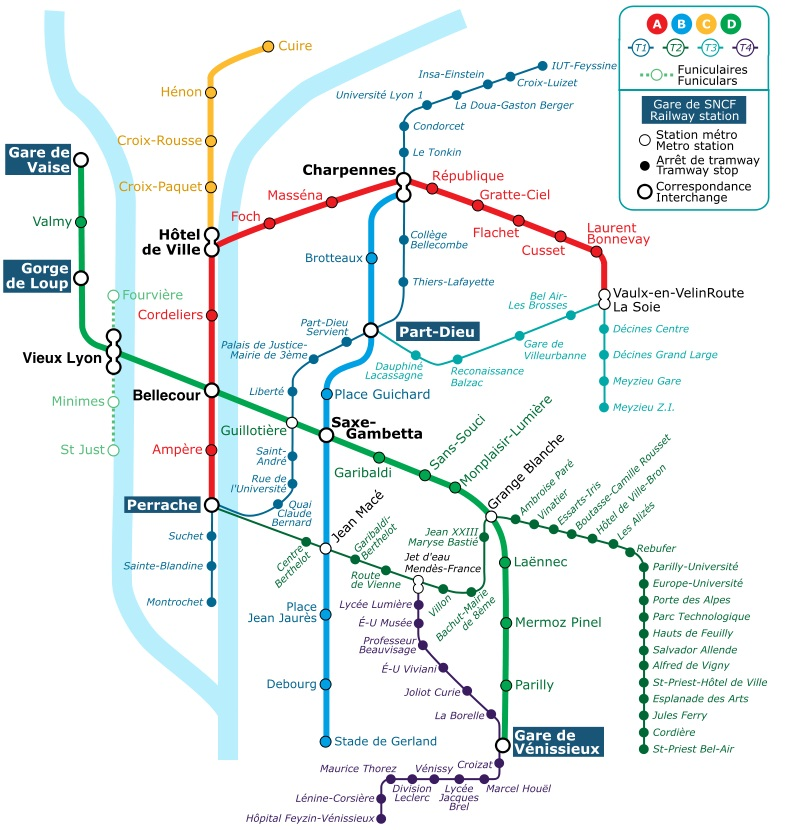
\includegraphics[scale=0.5]{Lyon.jpg}
            \caption{Mapa de la xarxa de metro de la ciutat de Lyon}
        \end{figure}

    \pagebreak

    \part{Treball previ a implementar l'algoritme \textit{A*}}
    \label{part:previ}

        \section{Exercici 2 - Expansió d’un node}
        \label{sec:Exercici2}

            Un primer pas per al nostre algoritme és expandir un node. Expandir vol dir que, donat un node, volem obtenir una llista amb els seus fills. Això, traduït a l’esquema de metro, ens diu a quines estacions podem anar des d’una estació donada, i per tant ens serveix per avançar per la xarxa.
            Cada node conté una llista amb els ID de les estacions adjacents. Si iterem sobre aquesta llista, podem construir-ne una nova amb els nodes que representen aquestes estacions, establint el node original com a pare, i acudint a la informació de la xarxa de metro per a obtenir les dades concretes de la estació (a partir de l’ID).
            Podem anar repetint aquesta expansió de forma cíclica, emprant els criteris adequats i filtrant-la amb les funcions pertinents, fins a formar una llista que acabarà esdevenint el camí òptim.

            A la vegada, aprofitem per establir certs valors addicionals de cada node, i que veurem més endavant, com son el cost real d’arribar fins al node, el cost heurístic i la funció d'avaluació (veure~\ref{subsec:CostRealNode}, \ref{sec:Exercici7} i \ref{sec:Exercici8}). Aquest valors tenen molta importància a l’algoritme, i per tant han de ser inclosos en tots els nodes.
            \begin{figure}[h]
                \centering    
                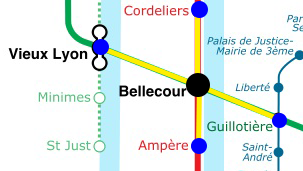
\includegraphics[scale=1]{expansion.png}
                \caption{Expansió del node negre. El resultat són els nodes blaus.}
            \end{figure}

        \section{Exercici 3 - Eliminar Cicles}
        \label{sec:Exercici3}

            Quan expandim un node, creem la llista amb totes les estacions adjacents. Això ens pot portar a situacions on, a la llista de fills, ens apareguin nodes ja expandits anteriorment. A aquest fenomen en diem cicle, i els cicles són contraproduents per al nostre algoritme, ja que el porta a entrar en bucles de camins (podem dir,que comença a fer voltes en cercles). És evident que un camí òptim no passa per aquest escenari, i per tant l’hem d’eliminar.

            Tots els nodes contenen una llista amb els ID de les estacions pare. Amb aquesta informació podem saber quins nodes son un cicle en una llista de nodes. Si per cada node de la llista, iterem sobre el conjunt d’IDs de pares, podem eliminar de la lista aquelles estacions que formen part del conjunt, deixant així la llista neta de cicles.
            \begin{figure}[h]
                \centering
                \begin{subfigure}[b]{0.3\textwidth}
                    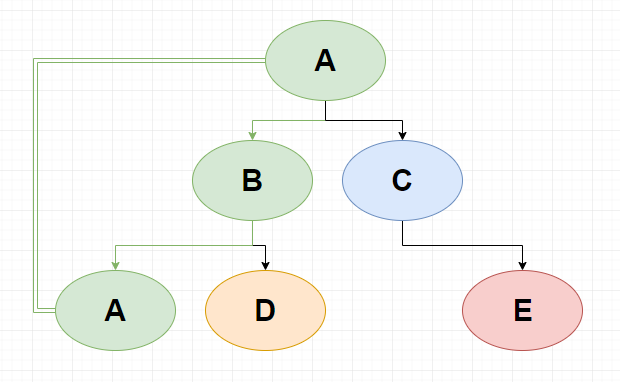
\includegraphics[width=\textwidth]{ciclo.png}
                    \caption{genèric}
                \end{subfigure}
                \hfil
                \begin{subfigure}[b]{0.3\textwidth}
                    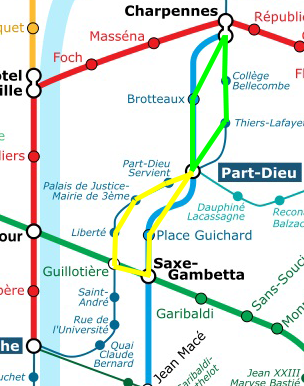
\includegraphics[width=\textwidth]{cicloLyon.png}
                    \caption{a la xarxa de Lyon.}
                \end{subfigure}
                \caption{Exemples de cicle}
            \end{figure}

        \section{Exercici 4 - Trobar l’estació més propera}
        \label{sec:Exercici4}

            Quan vulguem calcular la ruta entre dos punts, no sempre ens trobarem físicament a una estació de metro, així que una petita part del programa s’encarrega de trobar l’estació més propera a les coordenades indicades, a partir de la qual farà els càlculs. Malauradament, el programa no ens indica com arribar a aquesta estació més propera; això ja depèn de l’usuari.

            La idea és senzilla: com disposem de les coordenades de totes les estacions, podem crear una llista amb la distància euclidiana
            \begin{equation*} \label{eq:coord2station}
                dist_{(Coord,Station)} = \sqrt{(Coord_x - Station_x)^2 + (Coord_y - Station_y)^2}
            \end{equation*}
            entre el punt indicat i cadascuna de les estacions. Cada distància s’associa amb la ID de l’estació corresponent, i posteriorment aquesta llista s’ordena de menor a major distància. Finalment obtenim els ID de les estacions més properes (és a dir, els primers \textit{X} elements de la llista.
            Quan parlem de les \textit{X} primeres estacions de la llista ens referim a que podem tenir el cas de que tinguem més d’una estació exactament a la distància més propera, i per tant hem de recollir totes aquestes estacions.
            \begin{figure}[h]
                \centering    
                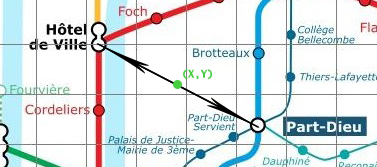
\includegraphics{distancias.png}
                \caption{Exemple de coordenades equidistants a dues estacions.}
            \end{figure}

        \section{Exercici 6 - Cost}
        \label{sec:Exercici6}

        En aquest exercici se'ns demana treballar sobre dos elements relacionats amb els costos: la taula de costos i el cost real d’un node.
        
            \subsection{Taula de costos}
            \label{subsec:Tauladecostos}

                Segons la preferència escollida per a calcular el trajecte, crearem una taula de costos basant-nos en la matriu d’adjacència (que forma part de la definició de la xarxa de metro). Aquesta matriu ens proporciona el temps que es triga entre una estació i una altra adjacent.
                Segons cada preferència, la taula de costos ens queda de les següents formes (com es calcula el valor per a cada element de la matriu):
                \begin{description}
                    \item[Adjacencia:] Si hi ha adjacència entre les estacions, l’element val 1; sinó val 0.
                    \item[Temps:] Com la matriu original està expressada en temps, la copiem directament per la taula de costos, i cada element expressa el temps entre estacions.
                    \item[Distància:] Disposem del temps entre estacions i de la velocitat de cada línia de la xarxa de metro (també forma part de la definició de la mateixa), per tant podem establir la distància com
                    \begin{equation*} \label{eq:cost_dist}
                        Cost_{Dist} = Time * LineVelocity
                    \end{equation*}
                    Cada element expressa aquest mateix càlcul.
                    \item[Transbords:] Si les dues estacions estan en línies diferents (i per tant hem de fer transbord per anar d’una a l’altra, l’element val 1; sinó val 0.
                    \item[Parades:] Una mateixa estació a nivell de xarxa de metro pot tenir més d’una estació a nivell de codi, ja que per cada línea en una estació de metro es genera una estació diferent a nivell de codi. En aquest cas ens interessa el primer tipus d’estació. Si les dues estacions tenen noms diferents (el nom no inclou la línia, i per tant representa el primer concepte) l’element val 1; sinó val 0. 
                \end{description}
            
            \subsection{Cost real d’un node}
            \label{subsec:CostRealNode}

                Cada node guarda, entre d’altres la dada del cost real. Aquest numero indica, segons la preferència escollida, quan ens ha costat arribar a aquell node des del node que designem com a origen del trajecte. Aixó es pot reinterpretar com: 
                \begin{equation*} \label{eq:realcost}
                    g_i = g_{i-1} + Cost(i-1, i)
                \end{equation*}
     
                Si partim de la taula de costos calculada a l’apartat anterior, i que el cost del node orígen és només el cost d’anar al següent node, podem calcular el cost real segons aquesta simple formula.
    
        \section{Exercici 7 - Heurístiques}
        \label{sec:Exercici7}

            Per poder determinar la funció de costos final, primer necessitem calcular la heurística adient segons la preferència que determini l’usuari.
            La heurística calculada, ha d’esdevenir admissible (mai ha de sobre-estimar el cost que falta per arribar a la solució).
            Segons la preferència que indiqui l’usuari, es tindran en compte una sèrie d’elements o no:
            \begin{description}
                \item[Mínim temps:] Per calcular l’heurística admissible depenent del temps, s’ha de tenir en compte si l’usuari es troba en una estació que comparteix línia amb l’estació de destí o no. En el millor dels casos, aquesta condició es complirà i per tant, aprofitant la fórmula
                \begin{equation*} \label{eq:velocity}
                    h_t = \frac{Dist}{MaxVelocity}
                \end{equation*}
                podem calcular el temps òptim aprofitant la velocitat màxima de la ciutat (que podem obtenir del paràmetre city que conté la informació de la ciutat).
                En cas contrari, a aquest temps òptim calculat, li haurem de sumar el temps que trigaria un usuari en realitzar un transbord.
                \item[Distància mínima:] Com ja hem esmentat, per tal que l’heurística sigui admissible, la manera que tenim de calcular aquesta, tenint en compte que la prioritat de l’usuari és obtenir el camí més curt, és utilitzar la distància en línia recta que hi ha entre les estacions d’origen i destí (aquest serà el cas òptim).
                \item[Mínim nombre de transbords:] En aquest cas, per determinar l’heurística, s’ha de comprovar si l’usuari es troba en la mateixa línia que l’estació de destí, de ser així, el millor cas és que l’usuari no ha de fer cap transbord, mentre que si no es compleix aquesta condició, l’usuari com a mínim (i per tant aquesta serà l’heurística que definirem) haurà de fer un transbord.
                \item[Mínim nombre de parades:] Per determinar el millor cas en quant a nombre de parades, hi ha dues possibilitats per a que l’heurística esdevingui admissible:
                \begin{enumerate}
                    \item L’estació d’origen sigui alhora la de destí (tot i que és una mica absurd).
                    \item L’estació de destí es trobi a una parada de distància respecte l’estació d’origen.
                \end{enumerate} 
            \end{description}
        
        \section{Exercici 8 - Funció heurística global}
        \label{sec:Exercici8}

            Un cop hem establert costos i heurístiques, hem de definir el que en diem la funció d'avaluació, que és realment el valor que utilitzarà l’algoritme \textit{A*} per tenir en compte els camins a escollir. El concepte és molt simple:
            \begin{align*}\label{eq:eval}
                EvalFunc &= Cost + Heuristic \\
                f &= g + h
            \end{align*}
            Podem interpretar-ho com que \textit{g} és una mirada al passat, i \textit{h} una predicció del futur. Junts ens donen una visió aproximada i optimista (perquè les heuristiques són admisibles) del cost total dels diferents camins possibles abans d’arribar al destí. D’aquesta, l’algoritme pot decantar-se per uns camins o altres amb més rapidesa que si no disposéssim d’aquesta predicció que és l’heurística.

        \section{Exercici 9 - Inserció ordenada}
        \label{sec:Exercici9}

            A l’hora de construir la nostra ruta óptima, l’algoritme \textit{A*} anirà generant una llista de nodes, on cada node és un camí (ja que podem traçar la llista de pares d’aquest node fins a l’origen). Ara bé, volem que l’algoritme analitzi sempre el camí amb menor cost acumulat, i per això necessitem una funció que ordeni aquesta llista en base a la funció d’avaluació \textit{f}.
            Ordenar la llista desde el valor \textit{f} menor (menor cost acumulat) fins al més gran.
            D’aquesta forma l’algoritme pot explorar sempre el primer camí de la llista de forma consistent, ja que sempre será el camí més òptim a priori, i no haurem de fer comprovacions intermitges.
        

        \section{Exercici 10 - Eliminar Camins Redundants}
        \label{sec:Exercici10}
        
            La idea darrera d’aquest exercici és simple, tot i que la execució ens ha costat una mica més d’entendre, al principi. Donada una llista de camins parcials, hi han alguns que són redundants i que no ens portaran a una solució òptima. Una forma d’eliminar camins redundants és eliminant cicles, com ja hem vist (\ref{sec:Exercici3}). Però ens trobem amb un altre cas, on anem del punt \textit{A} al \textit{B} (punts intermitjos de la ruta total) amb diferents, però hi ha un o més que són més òptims que els altres. Evidentment, els camins parcials no-optims (redundants) poden ser eliminats, ja que no ens portaràn a una un camí total óptim.
            \begin{figure}[h]
                \centering    
                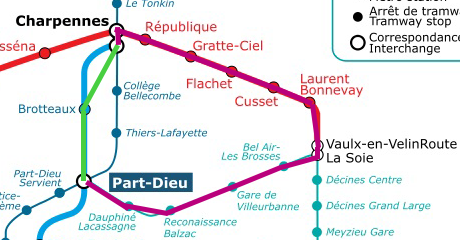
\includegraphics{redundantes.png}
                \caption{Exemple (molt exagerat), de camins redundants. En verd, camí òptim. En morat, camí redundant (molt més llarg, mateix origen i destí).}
            \end{figure}
            
            Per tal de poder comparar aquestes rutes intermitges i saber si son òptimes o no, a l’hora d’executar l’algoritme \textit{A*} mantindrem una llista de costos parcials, que ens diu quin ha estat el millor cost fins al moment per poder realitzar aquesta ruta. Amb aquesta taula podem procedir a la eliminació dels camins redundants.
            
            Hi ha 3 casos a valorar:
            \begin{itemize}
                \item \textbf{Si hi ha algun camí entre \textit{A} i \textit{B} més ràpid que els contemplats a la taula parcial de costos:} Actualitzem la taula, i eliminem la resta de camins que vagin entre aquest mateixos punts.
                \item \textbf{Si hi ha algun camí entre \textit{A} i \textit{B}, però és més lent que el contemplat a la taula parcial de costos:} Eliminem aquest camí, perquè és impossible que ens porti a una solució òptima.
                \item \textbf{El camí entre \textit{A} i \textit{B} mai ha estat explorat:} Afegim el seu cost a la taula parcial de costos.
            \end{itemize}

    \pagebreak
        
    \part{Implementant \textit{A*}}
    \label{part:astar}
    
        Un cop hem realitzat tots els exercicis previs, ja tenim totes les peces per a construir l’algoritme \textit{A*}. Explicarem els passos que hem seguit per implementar-lo, ja que hi ha petites variacions respecte el pseudocodi de l’enunciat.
        
        \begin{enumerate}
            \item Calcular la matriu de costos (veure~\ref{subsec:Tauladecostos}) segons la preferència escollida.
            \item Trobem les estacions més properes a les coordenades d'origen i destí (veure~\ref{sec:Exercici4}), generar els nodes corresponents i assignar els valors de cost real (veure~\ref{subsec:CostRealNode}), heurística (veure~\ref{sec:Exercici7}) i funció d’avaluació (veure~\ref{sec:Exercici8}).
            \item Apliquem el pseudocodi de l'enunciat, amb la diferència de que en comptes d’usar una llista de llistes (on la llista més interna és un camí amb els seus passos de forma explícita, i el seu cost al final), usem una llista de nodes (on cada node és un camí que ja conté totes les dades necessaries):
            \begin{figure}[h]
                \centering    
                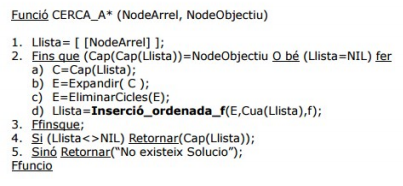
\includegraphics{pseudo.png}
                \caption{Pseudocodi de l'algoritme \textit{A*}}
            \end{figure}
        \end{enumerate}
    
        Un cop obtingut el node que conté el camí òptim, obtenim la llista amb les IDs que conformen la ruta òptima en sí, a partir de la llista (que està ordenada) de pares. Aquest és l’element clau de tot el programa. Aquesta llista és la solució al problema inicial.

        Desprès d'això tindrem en compte algunes mètriques addicionals:
        \begin{itemize}
            \item Al llarg de l’algoritme, hem anat mantenint una llista dels nodes visitats (de les seves IDs d’estació.
            \item Calculem a quina distància es troben les estacions escollides com a origen i destí de les coordenades proporcionades.
            \item Nombre de nodes visitats fins a arribar a la solució.
            \item Longitud (en nodes) del camí òptim.
        \end{itemize}
        
        Totes aquestes mètriques, juntament amb el camí final, es poden veure a la GUI proporcionada pels professors, que alhora serveix per carregar diferents xarxes de metro i fer les diferents consultes.

        \begin{figure}[h]
            \centering    
            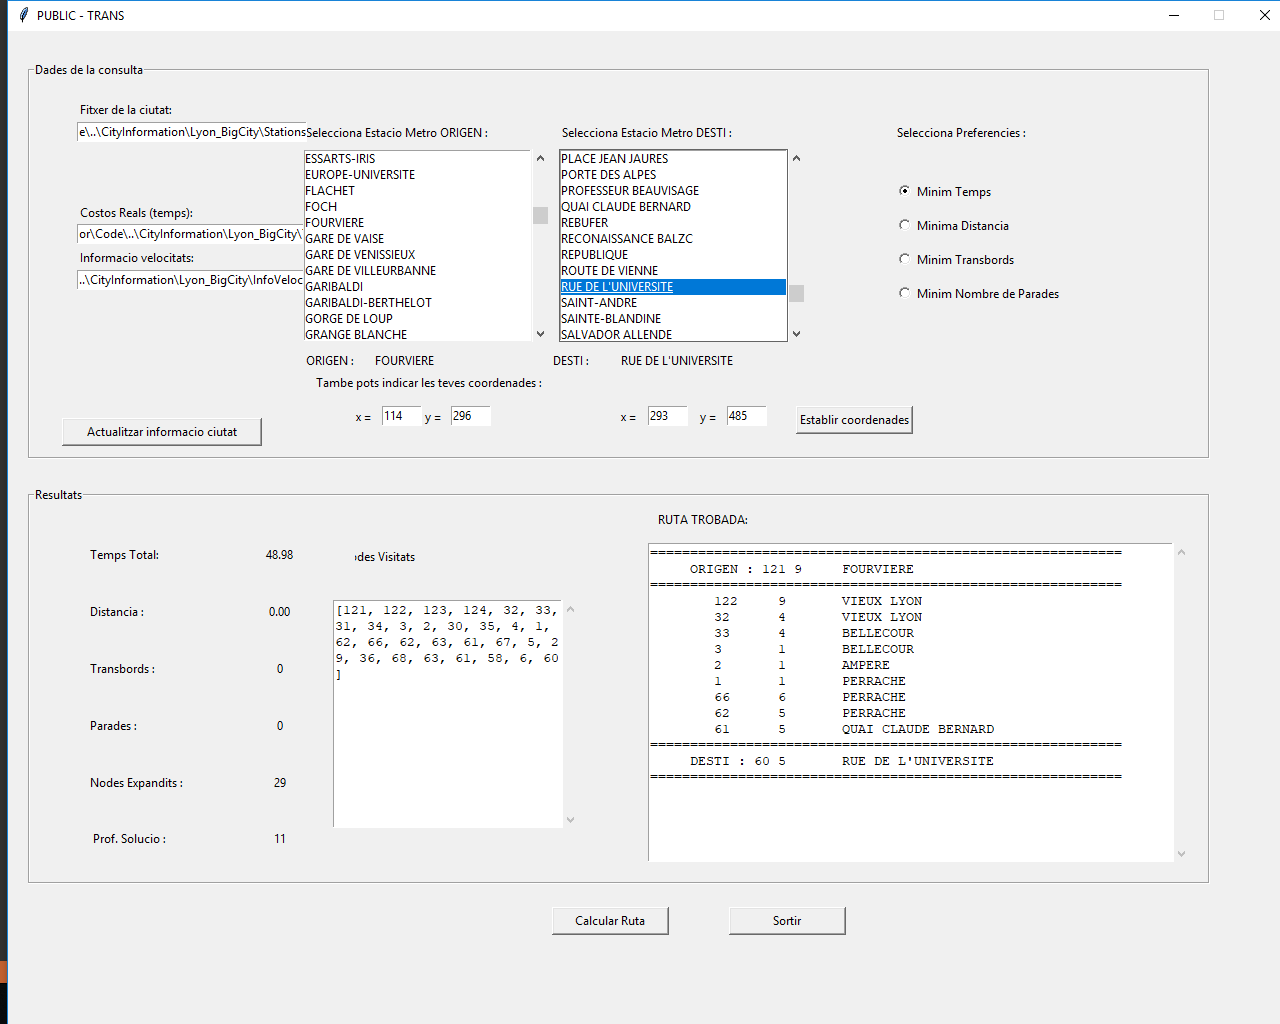
\includegraphics[scale=0.3]{consulta.png}
            \caption{Captura d'una consulta, amb el seus resultats.}
        \end{figure}

        Amb aquest apartat complet, la pràctica queda a punt per a ser testejada contra les consultes del guió, per tal de comprovar el correcte funcionament del programa amb les diferents casuístiques.
    
    \pagebreak
    
    \part{Conclusió}
    \label{part:conclusion}

    Després de testejar cada exercici, realitzar diverses consultes, i comprovar que els resultats coincideixen amb el joc de proves proporcionat, podem dir que la pràctica queda finalitzada.  Tenim un programa que compleix amb l’objectiu inicial: dir-nos com anar d’\textit{A} a \textit{B}, dins d’una xarxa de metro, segons la nostra preferència.

    Al llarg dels diferents apartats, hem pogut aprendre com funcionen les diverses parts que constitueixen l’algoritme \textit{A*}, com implementar-les, i com unir-les per tal de construir l’algoritme final. Certes parts han estat més difícils de plasmar que d’altres, com per exemple la dels camins redundants, però finalment hem pogut fer-les totes.
    Vam tenir certs problemes a l’hora de fer \textit{A*}, ja que el pseudocodi assumeix una representació de la informació que no és la emprada dins del codi real. (veure~\ref{part:astar})

    A part dels coneixements propis de l’assignatura, ens enduem dos reforços molt positius:
    \begin{itemize}
        \item Aquesta és el primer projecte de la carrera amb Python, i això ens ha obligat a posar-nos les piles amb el llenguatge. Al final del camí, podem dir que hem millorat certs aspectes de la programació Python, tot i que encara ens queda molt marge.
        \item A l’hora de realitzar aquesta memòria ens hem decantat per emprar \LaTeX, el sistema de composició de textos emprat mundialment per a documents formals. Ha estat la primera vegada que l'utilitzem, i certes coses han estat complicades, però el resultat final ha estat prou bo. Segurament continuem emprant aquesta eïna per a futurs treballs i informes.
    \end{itemize}
 
\end{document}